% Generated from ../chapters/01-the-river-and-the-machine.md
\chapter{The River and the Machine}\label{chapter-1-the-river-and-the-machine}

Modern medicine inherited one of the most productive metaphors in intellectual history: the body as a machine. Machines have parts. Parts wear, break, clog, and fail. Once the faulty part is identified, it can be repaired, replaced, or bypassed. The metaphor helped make anatomy precise and disease localizable. It prepared the way for surgery, intensive care, prosthetics, antibiotics, imaging, and molecular therapies.

The metaphor is powerful because bodies really do have components whose failure matters. A severed tendon cannot be talked back into continuity. An infection may require an antimicrobial. A blocked artery may require urgent intervention. Any systems account that denies these facts is not holistic; it is simply wrong.

Yet a living body is also unlike a machine in the property that matters most: it makes and remakes itself. An embryo does not arrive as a kit of parts assembled by an external engineer. Cells divide, migrate, differentiate, sense their neighbors, respond to force and electrical gradients, and collectively generate an anatomy. Adult tissues continue to turn over, repair boundaries, learn from loading, and change future responses. The body is made of parts, but its order is not imposed only from outside.

A river gives us a second metaphor. The same river persists while its water changes. Its identity lies in a pattern of flow constrained by a source, a gradient, a channel, a watershed, weather, organisms, and human activity. When a river becomes polluted, one can remove waste downstream. One can also go upstream, stop the source of pollution, reopen blocked channels, restore wetlands, and allow the river's own dynamics to carry sediment and renew habitats.

These are not competing strategies. A river sometimes needs direct engineering. But the upstream question is different from the mechanical one. Instead of asking only \emph{which damaged piece should be repaired?}, it asks \emph{which conditions keep recreating the damage?}

Consider chronic tension in the jaw and neck. A local examination may reveal dental pathology, joint degeneration, muscle spasm, or nerve irritation. Those findings matter. A systems examination additionally asks why the pattern is reproduced each day. Vision, breathing, threat prediction, sleep, habitual posture, pain avoidance, work, and social stress may all contribute. Treating one muscle can be useful while leaving the watershed untouched.

This is the first principle of the book:

\begin{quote}
\textbf{When a living system repeatedly recreates a problem, look not only for the defective component but for the organization that makes the problem stable.}
\end{quote}

The river will return throughout the book, but it should not be made to carry more than it can. A body is not literally water flowing through a channel. The metaphor serves one purpose: to shift attention from static components to processes that preserve identity through change. Once that shift is made, we need the more exact language of complex systems.

\begin{figure}
\centering
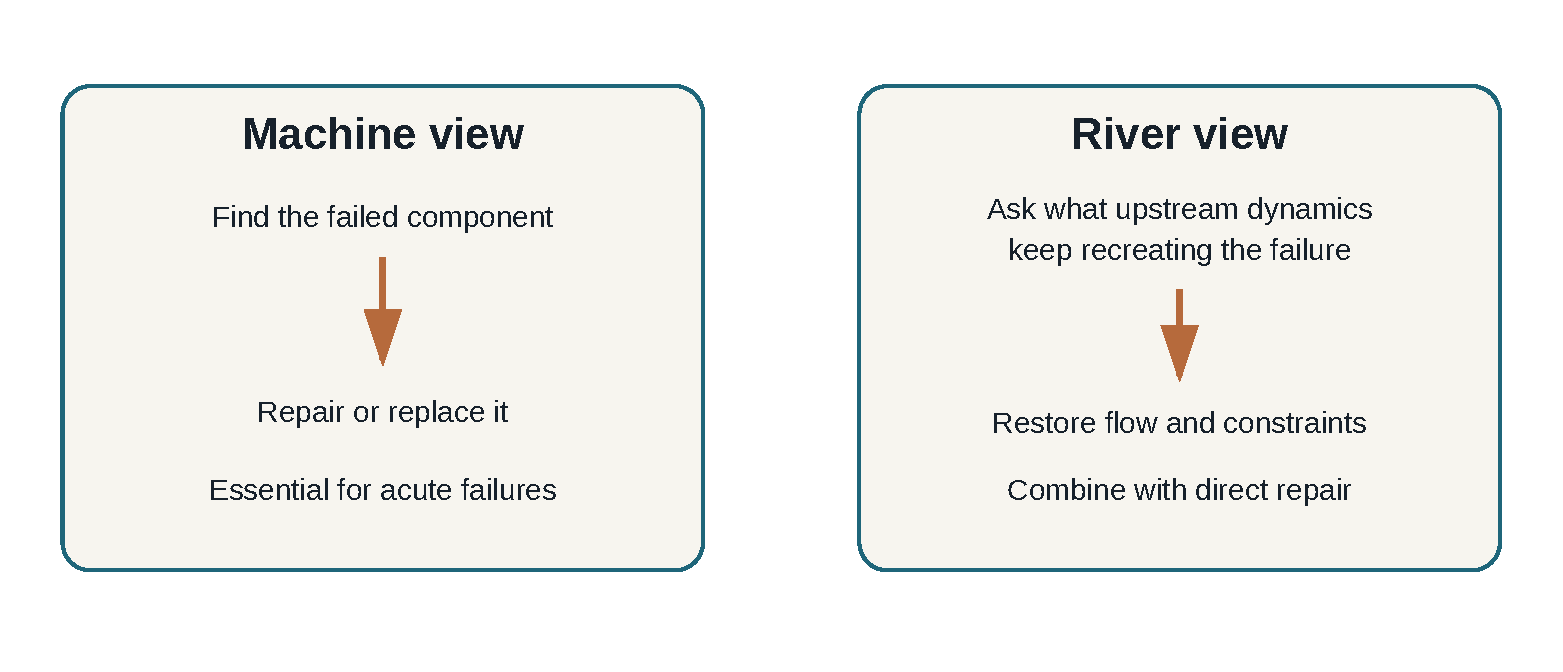
\includegraphics[width=0.92\textwidth,height=.68\textheight]{../figures/river-machine.pdf}
\caption{The machine asks which part failed; the river also asks which upstream dynamics keep recreating the failure.}\label{fig:river-machine}
\end{figure}

The conceptual lineage is broad. General systems theory argued that organization and relations could not always be understood by studying isolated components \autocite{bertalanffy1968general}. Autopoiesis described living systems as networks that continually produce the components and boundaries that constitute them \autocite{maturana1980autopoiesis}. Contemporary systems biology studies interactions, feedback, and network behavior rather than treating a molecular list as a complete explanation.

The machine metaphor remains indispensable. The error is to mistake an indispensable perspective for an exhaustive ontology. The body is a machine in some respects, a river in others, and finally something more demanding: a historically evolved, self-producing, multilayer adaptive system.
